\begin{enunciado}{\ejercicio}
Se define la siguiente relación $\relacion$ en $G_{20}$:
$$
  z\relacion w \sisolosi zw^9 \en G_2.
$$
\begin{enumerate}[label=\roman*)]
  \item Probar que $\relacion$ es una relación de equivalencia.
  \item Calcular la cantidad de elementos que hay en cada clase de equivalencia.
\end{enumerate}

\end{enunciado}

\begin{enumerate}[label=\roman*)]
  \item
        \textit{Reflexividad: }\par
        $ z = e^{i\frac{1}{10}\pi k_z}
          \entonces
          z \relacion z
          \sisolosi
          e^{i\frac{1}{10}\pi k_z} \cdot e^{i\frac{9}{10}\pi k_z} =
          e^{ik_z\pi } =
          \llave{rl}{
            1 & k_z \text{ par}\\
            -1 & k_z \text{ impar}\\
          } \Tilde
        $\par

        \textit{Simetría: }\par
        $ z = e^{i\frac{1}{10}\pi k_z}
          \text{ y }  w = e^{i\frac{1}{10}\pi k_w} \en G_{20}.$

        $\relacion$ es simétrica si:
        $z \relacion w
          \sisolosi w \relacion z\\
          \llave{l}{
          zw^9 = e^{i \frac{\pi}{10}(k_z + 9k_w)} \en G_2
          \sii
          \frac{1}{10}(k_z + 9k_w) = k
          \sii
          k_z + 9k_w = 10k
          \sii
          \congruencia{k_z}{-9k_w}{10}
          \sii
          \congruencia{k_z}{k_w}{10} \\
          \to
          \boxed{
            z\relacion w
            \sisolosi
            \congruencia{k_z}{k_w}{10}
          }\\

          wz^9 = e^{i \frac{\pi}{10}(k_w + 9\magenta{k_z})} =
          e^{i \frac{\pi}{10}(k_w + 9(\magenta{10k + k_w}))} =
              e^{i \frac{\pi}{10}(90k + 10k_w)} =
              e^{i (9k + k_w)\pi} =
              e^{i\blue{k'}\pi}\\
            }$\par
        $\boxed{z \relacion w \sisolosi w \relacion z}
          \paratodo k,\,k_w \en \enteros \text{ con } \congruencia{k_z}{k_w}{10}\Tilde$\par

        \textit{Transitividad: }\par
        $ \llaves{l}{
            z = e^{i\frac{1}{10}\pi k_z}\\
            w = e^{i\frac{1}{10}\pi k_w}\\
            y = e^{i\frac{1}{10}\pi k_y}
          } \en G_{20}
          \to
          \relacion$ es transitiva si:
        $z \relacion w  \text{ y } w\relacion y
          \entonces
          z \relacion y\\
          \llaves{l}{
            z \relacion w
            \sisolosi
            \congruencia{k_z}{k_w}{10} \llamada1\\
            w \relacion y
            \sisolosi
            \congruencia{k_w}{k_y}{10} \llamada2
          }\\
          \to
          zy^9 = e^{i \frac{\pi}{10}(\magenta{k_z} + 9k_y)} \igual{$\llamada 1$}
          e^{i \frac{\pi}{10}(\magenta{10 k + k_w} + 9k_y)} \igual{$\llamada 1$}
          e^{i \frac{\pi}{10}(10 k + 10k' + k_y + 9k_y)} =
          e^{i (k + k' + k_y) \pi}  =
          e^{i \blue{k''} \pi}
          \\
          \boxed{
            \llaves{l}{
              z \relacion w\\
              w \relacion z
            } \entonces z\relacion y}$

  \item $\# \clase{e^{i\frac{2\pi}{20} k}} = 2$ para algún $k \en \enteros / r_{20}(k) < 20$. Dada
        la condición $\congruencia{k_z}{k_w}{10}$, solo hay 2 números que tienen misma cifra de unidad
        entre 0 y 20. En el gráfico se ve que si $z\relacion w \entonces w = -z $
\end{enumerate}

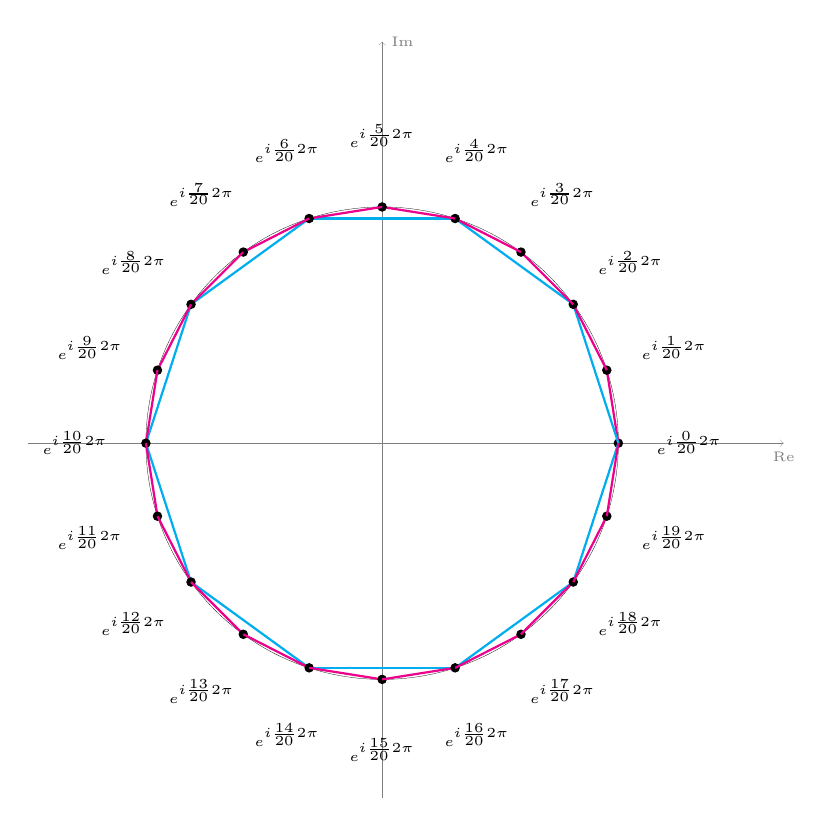
\begin{tikzpicture}[baseline=0,scale = 3, every node/.style={font=\tiny}]
  \draw[ultra thin,->,gray] (-1.5,0) -- (1.7,0) node[below] {Re};
  \draw[ultra thin,->,gray] (0,-1.5) -- (0,1.7) node[right] {Im};
  \draw[ultra thin] (0,0) circle (1);
  \foreach \x in {0,...,19} {
      \filldraw (\x*360/20:1) circle (0.5pt);
      \filldraw (\x*360/20:1.3) node { $e^{i\frac{\x}{20}2\pi}$};
      \ifnum\x<20
        \draw[thick, magenta] (\x*360/20:1) -- ({(\x+1)*360/20}:1);
      \fi
      \ifnum\x<10
        \draw[thick, cyan] (\x*360/10:1) -- ({(\x+1)*360/10}:1);
      \fi
    }
\end{tikzpicture}
